\documentclass[oneside,14pt]{extarticle}
\usepackage[utf8]{inputenc}
\usepackage[english,ukrainian]{babel}
\usepackage{amssymb,amsfonts,amsmath,amsthm,mathtext,textcomp}

\usepackage[includehead, headsep=0pt, footskip=0pt, top=2cm, bottom=2cm, left=2cm, right=2cm]{geometry}
\usepackage{indentfirst}
\usepackage[onehalfspacing]{setspace}
\usepackage[headings]{fancyhdr}
\usepackage{etoolbox}
\usepackage{flafter}
\usepackage{hyperref}
\usepackage{multirow}
\usepackage{listings}
\usepackage{graphicx}
\usepackage{float}
\usepackage[center]{titlesec}
\titlelabel{\thetitle.\quad}
\usepackage{array}
\fancyhf{}
\renewcommand{\headrulewidth}{0pt}
\renewcommand{\baselinestretch}{1.5}
\pagestyle{fancy}
\fancyfoot[R]{\thepage}
\lstset{breaklines=true,}
\graphicspath{ {./pictures} }
\counterwithin{figure}{section}

\begin{document}
\begin{titlepage}
	\begin{center}
МІНІСТЕРСТВО ОСВІТИ І НАУКИ УКРАЇНИ\\
НАЦІОНАЛЬНИЙ УНІВЕРСИТЕТ <<ЛЬВІВСЬКА ПОЛІТЕХНІКА>>\\
ННІ АДМІНІСТРУВАННЯ ТА ПІСЛЯДИПЛОМНОЇ ОСВІТИ\\
КАФЕДРА ТЕХНОЛОГІЙ УПРАВЛІННЯ

		
		\vspace{80pt}
Контрольна робота\\
з дисципліни <<Бізнес-планування та управління проектами>>\\
Варіант №55
\begin{flushleft}
	1 теор. пит. №1\\
	2 теор. пит. №14\\
	1 прак. зав. №5\\
	2 прак. зав. №7\\
\end{flushleft}
		\vspace*{20pt}
		
		\begin{flushright}
			\textbf{Виконав}:\\
			
			студент групи БПУ-ТУ-213\\
			Коваленко Д.М.\\
			\vspace{10pt}
			\textbf{Прийняла}:\\
			ст викл. Лебідь Т.В.
			
			\vspace{28pt}
			«\rule{1cm}{0.15mm}» \rule{1.5cm}{0.15mm} 2023 р.\\
			$\sum$ = \rule{1cm}{0.15mm}……………\\
			
		\end{flushright}
		\vspace{\fill}
		Львів — 2023
	\end{center}
\end{titlepage}
\setcounter{page}{2}
\tableofcontents
\newpage

\section*{ВСТУП}
\addcontentsline{toc}{section}{ВСТУП}
Метою виконання контрольної роботи є вивчення сучасної методико-прикла-дної бази бізнес-планування та управління проектами і програмами.

Навчальними завданнями є – вивчення наукових категорій, набуття практичних навиків визначення пріоритетного напряму діяльності бізнесу, розрахунку показників бізнес-плану та оформлення проектів його розділів, формування бізнес-плану, оцінювання економічної ефективності проектів, налагодження, розвитку та узгодження взаємодії зі стейкхолдерами у проектній діяльності, застосування методів фінансового планування та проектного бюджетування, визначення джерел фінансування, схем фінансування проектів. 

Окремими навчальними завданнями є набуття знань та розуміння параметрів і чинників впливу на розвиток проекту з метою формування його бюджету, ризиків проектної діяльності, методів керівництва проектами і програмами, зокрема фінансових ризиків проекту, їхнє врахування під час застосування бюджетного методу управління проектом, 

До навчальних завдань належить також набуття умінь самостійно працювати з навчальною, монографічною та періодичною літературою, оброблення та узагальнення, критичне аналізування даних наукових джерел, використання законодавчої та нормативної бази, набуття вмінь застосовувати методи дослідження та формулювати висновки відповідно до отриманих в результаті дослідження результатів.

\newpage
\section*{Теоретичне питання 1}
\addcontentsline{toc}{section}{Теоретичне питання 1}

Базові поняття управління проектами.

Управління проектами - це процес планування, організації, керування та контролю різних етапів проекту з метою досягнення його цілей у визначених обмеженнях, таких як обсяг робіт, терміни, витрати та якість. Існує кілька базових понять, які використовуються в управлінні проектами:
\begin{itemize}
	\item Проект - це унікальна задача або набір завдань, які виконуються один раз з метою досягнення конкретної мети. Проект має чітко визначені початок і кінець.
	\item Цілі проекту - це конкретні, вимірювані результати, які потрібно досягти в рамках проекту. Цілі повинні бути специфічними, досяжними, реалістичними, вимірюваними та часово обмеженими (метод SMART).
	\item Обсяг проекту - це повний перелік робіт, які повинні бути виконані для досягнення цілей проекту. Обсяг проекту включає всі завдання, ресурси, терміни та результати, які повинні бути враховані під час планування та виконання проекту.
	\item Терміни - це графік або розклад, який визначає часові рамки для виконання різних завдань і етапів проекту. Терміни допомагають планувати і контролювати прогрес проекту.
	\item Ресурси - це люди, матеріали, обладнання та фінансові ресурси, які необхідні для виконання проекту. Керування ресурсами включає планування, координацію та використання ресурсів в ефективний спосіб.
	\item Команда проекту - це група людей, які об'єднуються для виконання проекту. Кожен член команди має свої власні ролі, відповідальності та завдання, але працює в напрямку спільної мети.
	\item Ризики - це потенційні події або ситуації, які можуть вплинути на успішне завершення проекту. Управління ризиками включає ідентифікацію, аналіз та управління ризиками з метою зменшення негативних наслідків.
	\item Моніторинг та контроль - це систематичне спостереження за прогресом проекту, перевірка відповідності до поставлених цілей, виявлення відхилень та прийняття відповідних заходів для виправлення ситуації.
	\item Зацікавлені сторони (стейкхолдери) - це особи або організації, які мають інтерес у проекті або можуть бути безпосередньо або опосередковано задіяні в ньому. Вони можуть включати замовника проекту, команду проекту, клієнтів, постачальників, урядові органи, громадські організації та інші.
	\item Контрольні точки (milestones) - це ключові етапи або події в проекті, які вказують на досягнення певних результатів або проміжних цілей. Контрольні точки допомагають виміряти прогрес проекту, встановити пункти відліку і забезпечити відповідну комунікацію зі зацікавленими сторонами.
	\item Життєвий цикл проекту - це фази або етапи, через які проект проходить від початку до закінчення. Життєвий цикл може включати фази, такі як ініціація, планування, виконання та закриття. Кожна фаза має свої характеристики, завдання та результати.
	\item Завдання проекту - це конкретні дії, які потрібно виконати для досягнення цілей проекту. Завдання можуть бути розбиті на підзавдання, які призначаються різним членам команди проекту. Кожне завдання має визначену відповідальність, терміни виконання та взаємозв'язок з іншими завданнями.
	\item Комунікація - це обмін інформацією між учасниками проекту з метою передачі знань, координації робіт, вирішення проблем та забезпечення взаєморозуміння. Ефективна комунікація є ключовим елементом успіху проекту і може включати зустрічі, електронну пошту, звіти, презентації та інші засоби спілкування.
\end{itemize}

Ці поняття становлять основу управління проектами і допомагають керівникам проектів ефективно планувати, виконувати і контролювати проекти для досягнення бажаних результатів.

\newpage
\section*{Теоретичне питання 2}
\addcontentsline{toc}{section}{Теоретичне питання 2}

Характеристика організаційної структури бізнесу.

Організаційна структура бізнесу - це система, що визначає, як функції, відділи та посади взаємодіють між собою в межах підприємства. Вона визначає ланцюг командування, рівні влади, комунікаційні шляхи та відносини між працівниками. Організаційна структура відображає формальні інформаційні потоки, зв'язки та ієрархію в організації. Основні характеристики організаційної структури бізнесу включають:

\begin{itemize}
	\item Функціональна структура: Це найпоширеніший тип організаційної структури, при якому підприємство поділяється на функціональні відділи, такі як виробництво, маркетинг, фінанси, персонал і т. д. Кожен відділ спеціалізується на конкретній функції, а співробітники підпорядковуються керівникам відповідних відділів. Цей тип структури сприяє ефективному управлінню та спеціалізації, але може призводити до вузького спеціалізованого підходу та погіршення комунікації між відділами.
	\item Дивізіональна структура: В цьому типі структури організація розділяється на дивізіони або підрозділи, які функціонують як самостійні одиниці з власними відділами функцій, такими як продажі, виробництво, маркетинг, управління персоналом і т. д. Кожен дивізіон може мати свою власну структуру, яка відповідає його потребам. Цей підхід дозволяє краще враховувати потреби різних ринків або продуктів, але може призводити до дублювання ресурсів і складнішого управління.
	\item Матрична структура: Цей тип структури поєднує функціональну і дивізіональну структури, де працівники мають дві або більше лінії підпорядкування. Наприклад, проектні команди можуть складатися з фахівців з різних відділів, які працюють над конкретними проектами. Це забезпечує гнучкість та швидкість реагування на зміни, але може виникати конфлікти між лінійною та проектною структурами.
	\item Сіткова (мережева) структура: Цей тип структури використовується в основному для проектних команд або в організаціях, де співробітники працюють над різними проектами. Всі члени команди співпрацюють безпосередньо між собою і мають велику самостійність. Цей підхід сприяє гнучкості, творчості та інноваціям, але може призводити до відсутності чіткої лінії командування та ускладнення координації.
	\item Централізована та децентралізована структури: Централізована структура передбачає, що влада та прийняття рішень зосереджені у вищих рівнях організації, таких як власник, генеральний директор або виконавчий комітет. У децентралізованій структурі влада та прийняття рішень розподілені між різними рівнями та підрозділами організації. Децентралізація сприяє швидкій реакції, більшій відповідальності та залученню працівників до процесу прийняття рішень.
	\item Горизонтальна та вертикальна структури: У вертикальній структурі організації існує ієрархічна ланка командування від верхнього рівня до нижнього. У горизонтальній структурі наголошується на співпраці та колаборації між різними відділами чи функціональними групами. Горизонтальна структура сприяє швидкій комунікації, обміну ідеями та інноваціям.
	\item Географічна структура: У такій структурі організація поділяється на географічні регіони або місця, де філії або відділення відповідають за свої власні ринки чи території. Кожен регіон має свої власні функції та відповідальності, але може бути координація та співпраця між ними.
	\item Процесно-орієнтована структура: У такій структурі організація фокусується на процесах, які лежать в основі її діяльності. Кожен процес має свої власні відповідальності та ресурси, а співробітники можуть бути призначені для роботи над певними процесами з різних функціональних відділів.
\end{itemize}

Ці характеристики організаційної структури можуть варіюватися в залежності від конкретної організації та її потреб. Важливо підкреслити, що організаційна структура повинна відповідати стратегії та цілям організації, сприяти ефективності та співпраці між працівниками та взаємодії зовнішніх стейкхолдерів.

\newpage
\section*{Практичне завдання 1}
\addcontentsline{toc}{section}{Практичне завдання 1}

Бюджет проекту 9 млн. грн. (без урахування фінансових витрат). Підприємство планує фінансування проекту повністю за рахунок кредиту. Термін кредитування 3 місяці, процентна ставка 25\% річних. Умовою кредитної угоди передбачено: 1) погашення тіла кредиту щомісячними рівними платежами; 2) щомісячна сплата процентів за кредитом. Дохід від реалізації проекту становить 15 млн. грн. Початок терміну кредитування 01.01 поточного року. Визначити витрати підприємства на фінансування проекту, скласти звіт про рух грошових коштів на фінансування витрат за проектом та визначити прибуток від реалізації проекту.

Розв'язання:
\begin{gather}
	r=3\text{ - термін кредитування в місяцях, }1/4\text{ - в роках}\nonumber\\
	I=L\cdot\frac{i\cdot r}{100}\nonumber\\
	9\cdot\frac{25\cdot (1/4)}{100}=0.5652\text{ млн. грн. - плата за користування кредитом}\nonumber\\
	S=I+L\nonumber\\
	9+0.5652=9.5652\text{ млн. грн. - сума кредиту}\nonumber\\
	15-9.5652=5.4348\text{ млн. грн. - прибуток від реалізації проекту}\nonumber
\end{gather}

\begin{table}[h]
	\centering
	\caption{Звіт про рух грошових коштів на фінансування витрат за проектом}
	\renewcommand{\arraystretch}{1.3}
	\begin{tabular}{|c|c|c|}
		\hline
		\textbf{Період} & \textbf{Тіло кредиту} & \textbf{Проценти} \\
		\hline
		01.01 & 3 млн. грн. & 0.1884 млн. грн. \\
		\hline
		01.02 & 3 млн. грн. & 0.1884 млн. грн. \\
		\hline
		01.03 & 3 млн. грн. & 0.1884 млн. грн. \\
		\hline
	\end{tabular}
\end{table}


\newpage
\section*{Практичне завдання 2}
\addcontentsline{toc}{section}{Практичне завдання 2}

Для проекту створення коворкінг-центру до основних ризиків віднесено: технічні – викликані необхідністю переобладнання приміщень; фінансові – викликані нестабільністю фінансової системи; кадрові – викликані необхідністю залучення фахівців відповідної кваліфікації; організаційні – викликані необхідністю формування інтелектуального простору співтворення. Експертна група встановила кількісні характеристики ризику проекту – ймовірність настання, ступінь впливу на реалізацію проекту (табл. 1). Необхідно позиціонувати ризики на графічній моделі матриці ризиків та вибрати стратегії управління ризиками.

Розв'язання

\begin{table}[h]
	\centering
	\renewcommand{\arraystretch}{1.3}
	\caption{Кількісні характеристики ризику проекту}
	\begin{tabular}{|c|c|c|c|}
		\hline
		\textbf{№ з/п} & \textbf{Вид ризику} & \textbf{Ймовірність настання} & \textbf{Ступінь впливу} \\
		\hline
		1 & Технічний & 0.4 & 0.4 \\
		\hline
		2 & Фінансовий & 0.4 & 0.7 \\
		\hline
		3 & Кадровий & 0.8 & 0.3 \\
		\hline
		4 & Організаційний & 0.3 & 0.6 \\
		\hline
	\end{tabular}
\end{table}

\begin{figure}[H]
	\centering
	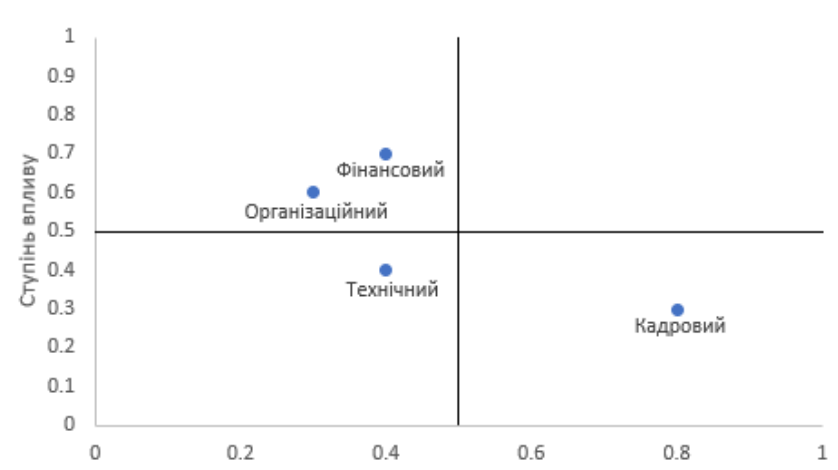
\includegraphics[width=\textwidth]{1}
\end{figure}

Технічні ризики позиціонуються у першому квадранті, тому підлягають
прийняттю. Це означає, що технічні менеджери принципово згодні з можливою
необхідністю переобладнання приміщень.
Фінансові та організаційні ризики позиціонуються у квадранті 2, тобто
стосовно них можна застосовувати стратегію регулювання (передачі) ризику:

\begin{itemize}
	\item стосовно фінансових ризиків – залучення до укладення лізингової
	угоди компетентних юристів (організацій).
	\item стосовно організаційних ризиків – залучення до формування
	інтелектуального простору співтворення спеціалізованих організацій.
\end{itemize} 

Кадрові ризики позиціонуються у четвертому квадранті. Це означає, що для
їх регулювання доцільно обрати стратегію запобігання ризику шляхом здійснення
превентивних заходів, спрямованих на недопущення ризикових ситуацій або
зведення до мінімуму ймовірності їх настання.

\newpage
\section*{СПИСОК ВИКОРИСТАНИХ ДЖЕРЕЛ}
\addcontentsline{toc}{section}{Список використаної джерел}

\begin{enumerate}
	\item ISO 3100:2018 Risk management. Guidelines. –Second edition. – 2018-02. – 24 pp.
	\item Чумаченко І. В. Управління проектами: процеси планування проектних дій / І. В. Чумаченко, В. В. Морозов, І. В. Доценко та ін. – К.: Університет економіки та права «Крок», 2014. – 673 с.
	\item Фещур Р. В. Прийняття проектних рішень: навч. посіб. / Р. В. Фещур, В. П. Кічор, А. І. Якимів [та ін.]; за ред. Р. В. Фещура. – Львів : Вид-во Львівської політехніки, 2013. – 216 с.
	\item Крикавський Є. Промисловий маркетинг: підручник. 2-ге вид. / Є.Крикавський, Н. Чухрай. – Львів: Видавництво Національного університету «Львівська політехніка», 2004. – 472 с.
	\item Маркетинг: підручник /А.О. Старостіна, Н.П. Гончарова, Є.В. Крикавський [та ін.]; за ред. А.О. Старостіної. – К.: Знання, 2009. – 1070с.
\end{enumerate}

\end{document}
